\documentclass[modern, trackchanges, dvipsnames]{aastex631}
  \urlstyle{sf}


\usepackage{CJK}
\usepackage{microtype}
\usepackage{savesym}
  \savesymbol{lambdabar}
\usepackage{newpxtext, eulerpx}
  \restoresymbol{newpx}{lambdabar}
\usepackage[T1]{fontenc}
\usepackage{fontawesome}
\usepackage{amsmath}
\usepackage{bm}
\usepackage{nicefrac}
\usepackage[caption=false]{subfig}
\usepackage[figure,figure*]{hypcap}
\usepackage{tikz}
 \usetikzlibrary{positioning, fit, calc, arrows.meta}
\usepackage{booktabs}
\usepackage{framed}


\newcommand{\pmwd}{{\usefont{T1}{nova}{m}{sl}pmwd}}
\newcommand{\GADGET}{{{\fontsize{10pt}{12pt}\selectfont GADGET}-4}}
\newcommand{\GSDATA}{{GS512}}

\renewcommand{\sectionautorefname}{Sec.}
\renewcommand{\subsectionautorefname}{Sec.}
\renewcommand{\appendixautorefname}{App.}
\renewcommand{\figureautorefname}{Fig.}
\newcommand{\subfigureautorefname}{\figureautorefname}

%FIXME copied from ../adjoint/adjoint.tex
\newcommand{\deltaD}{\delta^\textsc{d}}
\newcommand{\deltaK}{\delta^\textsc{k}}
\renewcommand{\d}{d}
\newcommand{\p}{\partial}
\newcommand{\cJ}{\mathcal{J}}
\newcommand{\cR}{\mathcal{R}}
\newcommand{\cL}{\mathcal{L}}
\newcommand{\cH}{\mathcal{H}}
\bmdefine{\vzero}{0}
\bmdefine{\vI}{I}
\bmdefine{\vnabla}{\nabla}
\bmdefine{\vtheta}{\theta}  % parameters
\bmdefine{\vvartheta}{\vartheta}  % relevant scales and factors to form
                                  % dimensionless features as NN inputs
\bmdefine{\vomega}{\omega}  % white noise modes
\bmdefine{\vk}{k}  % wavevectors
\bmdefine{\vx}{x}  % comoving and canonical coordinates
\bmdefine{\vq}{q}  % Lagrangian coordinates
\bmdefine{\vs}{s}  % displacements
\bmdefine{\vp}{p}  % canonical momenta
\bmdefine{\vv}{v}  % FIXME some velocities
\bmdefine{\va}{a}  % accelerations
\bmdefine{\vz}{z}  % states
\bmdefine{\vo}{o}  % observable
\bmdefine{\vmu}{\mu}  % observable adjoint
\bmdefine{\vO}{O}
\bmdefine{\vf}{f}
\bmdefine{\vF}{F}
\bmdefine{\vDelta}{\Delta}
\bmdefine{\vLambda}{\Lambda}
\bmdefine{\vlambda}{\lambda}
\bmdefine{\vvarphi}{\varphi}
\bmdefine{\vxi}{\xi}  % x adjoint
\bmdefine{\vpi}{\pi}  % p adjoint
\bmdefine{\valpha}{\alpha}  % force vjp x gradient
\bmdefine{\vzeta}{\zeta}  % force vjp theta gradient
\bmdefine{\vnu}{\nu}  % sensitivity
\newcommand{\lna}{\ln\!a}
\newcommand{\lnk}{\ln\!k}
\newcommand{\half}{\nicefrac12}
\newcommand{\As}{A_\mathrm{s}}
\newcommand{\ns}{n_\mathrm{s}}
\newcommand{\Omegam}{\Omega_\mathrm{m}}
\newcommand{\Omegab}{\Omega_\mathrm{b}}
\newcommand{\OmegaK}{\Omega_K}
\newcommand{\Mpc}{\mathrm{Mpc}}
\newcommand{\ic}{\mathrm{i}}
\newcommand{\f}{\mathrm{f}}
\newcommand{\linear}{\mathrm{lin}}
\newcommand{\tophat}{\mathrm{TH}}
\newcommand{\gauss}{\mathrm{G}}

\newcommand{\GPU}{NVIDIA H100 PCIe}  % 80GB memory

\newcommand{\YL}[1]{\textcolor{Bittersweet}{#1}}
\newcommand{\YZ}[1]{\textcolor{MidnightBlue}{#1}}



\begin{document}



\title{\large Neural and Symbolic Optimization of Cosmological
Particle-Mesh Simulation
\vspace{0.3em}}


\author[0000-0002-9300-2632]{\normalsize Yucheng Zhang}
\affiliation{Pengcheng Laboratory, Shenzhen, Guangdong 518066, China}
\affiliation{Center for Cosmology and Particle Physics, New York
University, New York, New York 10003, USA}

\author[0000-0002-0701-1410]{\normalsize Yin Li}
\affiliation{Center for Computational Mathematics, Flatiron Institute,
New York, New York 10010, USA}
\affiliation{Pengcheng Laboratory, Shenzhen, Guangdong 518066, China}
\affiliation{Center for Computational Astrophysics, Flatiron Institute,
New York, New York 10010, USA}

\author[0000-0001-5044-7204]{\normalsize Drew Jamieson}
\affiliation{Max Planck Institute for Astrophysics, 85748 Garching bei
M\"unchen, Germany}

\author[0000-0003-0745-9431]{\normalsize Libin Lu}
\affiliation{Center for Computational Mathematics, Flatiron Institute,
New York, New York 10010, USA}

% \author{\normalsize Heung-Yeung Shum}
% \affiliation{International Digital Economy Academy, Shenzhen, Guangdong
% 518000, China}
% \affiliation{Tsinghua University, Beijing 100084, China}
% \affiliation{The Hong Kong University of Science and Technology,
% Hong Kong 999077, China}


\shorttitle{Optimized Cosmological Simulation}
\shortauthors{Zhang \& Li et al.}


\correspondingauthor{Yucheng Zhang \& Yin Li}
\email{yucheng.zhang@nyu.edu \& eelregit@gmail.com}



\begin{abstract}
% up to 150 words

We optimize the spatial resolution of cosmological particle-mesh (PM)
simulations by sharpening the PM force with first neural networks (NNs)
and then symbolic regression (SR), taking symmetry and dimensional
analysis in consideration.
We embed deep NNs in the differentiable cosmological $N$-body
simulation, and training them to learn for the force kernel.
We fit the trained NNs with SR to extract an analytic kernel for better
interpretability and physical insights, which is also applicable to all
other cosmological PM simulation code.

\end{abstract}


% Main text: up to 3500 words: introduction + results + discussion
\vspace{1em}
\section{Introduction}
\label{sec:intro}
% without heading

% AI for science and cosmology
Rapid advances in artificial intelligence (AI) and more specifically
deep learning have provided powerful tools that are revolutionizing
scientific research across disciplines.
AI for science benefits from not only the state-of-art architectures of
deep neural networks (NNs), but also more fundamental computational
tools and hardwares like automatic differentiation (AD) and GPUs.
One of the very promising areas of AI in cosmology is the numerical
simulation of the Universe.

% a brief review of (differentiable) cosmological simulations
% BORG, ELUCID, and BORG-PM \citep{BORG, ELUCID, BORG-PM}
% \texttt{FastPM} and \texttt{FlowPM} \citep{FastPM, vmad, SeljakEtAl2017, FlowPM}

Cosmological $N$-body simulations evolve dark matter particles under the
gravitational interaction, which at the field level is described by the
Poisson equation
%
\begin{equation}
  \nabla^2 \varphi(\vx) = \frac32 \Omegam H_0^2 \delta(\vx),
\end{equation}
%
where $\Omegam$ is the matter fraction today, $H_0$ is the Hubble
constant, and the two fields $\varphi(\vx)$ and $\delta(\vx)$ are the
gravitational potential and matter density fluctuation respectively.
In Fourier space, the gravitational force field $\vF = - \vnabla
\varphi$ follows
%
\begin{equation}
\vF(\vk) = i \frac32 \Omegam H_0^2 \,\frac{\vk}{k^2} \delta(\vk),
\label{force}
\end{equation}
%
where the Laplacian operator reduces to simple multiplications of the
wavevectors.
The force field in configuration space $\vF(\vx)$ can then be recovered
with an inverse Fourier transform of $\vF(\vk)$.
The particle-mesh (PM) method is a fundamental and efficient approach to
solving the Poisson equation in the $N$-body simulation.
In order to perform the transformation between configuration and Fourier
spaces efficiently using the fast Fourier transform (FFT), PM estimates
the matter density field on a regular grid by scattering the particles
onto an auxiliary mesh.
The cloud-in-cell (CIC), or trilinear, interpolation scheme
\citep{HockneyEastwood1988} has been widely used to compute the mass
fractions of a particle at $\vx'$ scattered to a nearby mesh point
at $\vx$
%
\begin{equation}
  W(\vx, \vx') = \prod_{i=1}^3
    \max \Bigl( 1 - \frac{|x_i-x'_i|}{l_c}, 0 \Bigr),
  \label{cic}
  \end{equation}
%
where $l_c$ is the mesh cell size.
Other scattering schemes include the nearest grid point (NGP) and
triangle shaped cloud (TSC) etc.
The gravitational force field is evaluated in the Fourier space and
transformed back to the configuration space on the mesh points, which
are then grathered to form the interpolated force for each particle,
with the same weights as in the scattering process.
Although being computationally efficient, the accuracy of the
gravitational force estimated for each particle depends on the
resolution of the mesh.
The PM method is mainly limited by its accuracy on small scales around
and below the mesh cell size, due to the loss of information during the
scattering and gathering process between the continuously distributed
particles and the regular discrete mesh.

In this work, we perform the spatial optimization (SO) of the PM
simulation by sharpening the gravitational force.
We embed NNs in the force equation \eqref{force} and train them towards
the targets that are more accurate on small scales.
NNs are flexible and efficient universal function approximators
\citep{Hornik1989}, which can be used to learn physical processes in
numerical simulations.
It is necessary for the simulations to be differentiable in order to
train the NNs with gradient based optimizers \citep[e.g.][]{Adam}.
We develop our training pipeline of the SO NNs in the framework of
the differentiable cosmological simulation with adjoint method
\citep{Li2022a} and the corresponding PM $N$-body library \pmwd\
\citep{Li2022b}.
To gain further physical insights into the PM method, we fit the trained
NNs using symbolic regression (SR).
Optimizing the accuracy of fast and differentiable simulations like
\pmwd\ is crucial for their applications in, e.g. generation of mocks
for cosmological surveys, simulation-based inference or field-level
inference.



\vspace{1em}
\section{Results}
% Results should be divided by topical subheadings
% Put main ideas in Results first, then more technical details in Methods.

\subsection{Optimization of Dynamics}

To improve the accuracy of the PM solver, we introduce SO force
sharpening by modifying the gravitational force equation \eqref{force}
to
%
\begin{equation}
F(\vk)_i = i \frac32 \Omegam H_0^2 \,\frac{k_i}{k^2}\,
                    f(k_i; \vvartheta) g(\vk; \vvartheta) \delta(\vk),
\label{force_so}
\end{equation}
%
where $f$ and $g$ are nonlinear functions of the wavevector components
and all possible relevant features $\vvartheta$, which are approximated
with NNs.
$k_i$ is a component of $\vk$, with $i\in\{1,2,3\}$ denoting the 3
principal axes of the simulation box.
Gravity obeys the $\mathrm{O}(3)$ rotational symmetry, which is however
broken by the PM solver to the O\textsubscript{h} discrete symmetry with
48 elements involving permutations and reversals of the 3 principal axes
of the simulation box.
The PM evaluation of each force component can further break the symmetry
along that axis, leaving the remaining 2 permutationally symmetric.
Therefore, we implement $f$ and $g$ to be even functions of the
wavevector components, and $g$ to be permutation equivariant in all 3
components, so that $f g$ is the most general modification to the force
kernel.
An even and real kernel in configuration space is also even in Fourier
space.
We take the absolute value of the wavevectors for the evenness, and sort
the 3 wavevector compontents to achieve the permutation equivariance.

For both the $f$ and $g$, their input features consist of tabular data,
therefore we adopt neural networks with fully connected layers, aka
multilayer perceptrons (MLPs) to learn the nonlinear functions.
Both $f$ and $g$ networks have $XXX$ hidden layers with $XXX\times
n_{\rm input}$ nodes for each layer, where $n_{\rm input}$ is the size
of the input layer, which is [...] and [...] for $f$ and $g$
respectively.
The rectified linear unit (ReLU) activation function is used for hidden
layers.
We further apply the exponential function to the output as a regulator
for positive output.
Being embedded in the differentiable simulation library \pmwd, the NNs
can be trained using gradient-based optimization methods as in usual
deep learning tasks.
The parameters of the NNs, which enter the force evaluation in every
time integration step, can be treated just the same as other
cosmological parameters.
The objective gradients are accumulated as discussed in
\autoref{sec:diffsim_obs}, based on which the parameters are then
optimized.


\subsection{Target Simulation and Data}

\begin{table*}
  \centering
  \caption{Ranges of \GADGET\ and \pmwd\ configurations and cosmological
  parameters.
  Note that the grid ratio need next fast len to determine the mesh shape
  for fast FFT.
  Given the box size, the mesh shape determines the cell size.
  The softening parameter gives the ratio of the comoving softening length
  to the mean particle spacing.
  The curvature $\OmegaK$ is related to the separate universe simulation.
  We sample parameters applicable to \GADGET\ during data generation, and
  those applicable to \pmwd\ during training.
  \YL{(I forgot why I wanted to sample mesh shape and mesh cell size...
  Now it seems more natural to me to have the ptcl spacing sampled
  uniformly instead...)}
  }
  \label{tab:param}
  \begin{tabular}{lcccr}
  \toprule
  applicability & parameter & distribution & range & sampling \\
  \midrule
  & $128^3$ white noise & $\mathcal{N}(\vzero, \vI)$ & 512 realizations & MC \\
  \cmidrule(lr){2-5}
  & box size in Mpc$/h$ & \YL{log-uniform} & [25.6, 2560) \\
  \cmidrule(lr){2-4}
  & snapshot offset & uniform & (0, 1] \\
  \cmidrule(lr){2-4}
  \GADGET\ & $\As \times 10^9$ & log-uniform & [1, 4) \\
  \cmidrule(lr){2-4}
  \& \pmwd\ & $\ns$ & log-uniform & [0.75, 1.25) & RQMC \\
  \cmidrule(lr){2-4}
  & $\Omegam$ & log-uniform & [1/5, 1/2) & see \autoref{fig:sobol} \\
  \cmidrule(lr){2-4}
  & $\Omegab / \Omegam$ & log-uniform & [1/8, 1/4) \\
  \cmidrule(lr){2-4}
  & $\OmegaK / (1 - \OmegaK)$ & uniform & [-1/3, 1/3) \\
  \cmidrule(lr){2-4}
  & $h$ & log-uniform & [0.5, 1) \\
  \cmidrule(lr){1-4}
  \GADGET\ & softening ratio & log-uniform & [1/50, 1/20) \\
  \cmidrule(lr){1-5}
  \pmwd\ & mesh shape & log-uniform & [128, 512] & MC \\
  \cmidrule(lr){2-4}
  \cmidrule(lr){1-4}
  training & loss grid offset & uniform & $[0, 1)^3$ \\
  \bottomrule
  \end{tabular}
  \end{table*}

Our target data samples are generated with the \GADGET\ simulation code
\citep{GADGET-4}, configured with high force accuracy settings.
We run 512 \GADGET\ simulations that cover a wide range of
configurations and cosmological parameters, as listed in
\autoref{tab:param}.
\YL{
Each simulation evolves $128^3$ particles from the initial time $a_\ic$
to the final time $a_\f=1$, saving 64 snapshots linearly spaced in scale
factor from $a_\ic + \gamma \Delta a$ to $1 - (1 - \gamma) \Delta a$.
We determine $a_\ic$ for each configuration depending on its cosmology
and mean particle spacing \citep{MichauxEtAl2021}, \YL{(YL elaborate why
and how here.)} which then sets the snapshot spacing $\Delta a = (1 -
a_\ic) / 64$.
To sample different alignment between the snapshots and the start/stop
times and avoid possible related numerical errors in \pmwd, we introduce
a fractional random offset $\gamma$ that varies between 0 and 1 for
different simulations.
}
The curvature $\OmegaK$ is related to the separate universe simulation
\citep{LiEtAl2014, WagnerEtAl2015}.
We refer to this training dataset of 512 \GADGET\ simulations
sampled with Sobol sequence as \GSDATA.
On average each \GADGET\ simulation takes roughly 2K CPU hours to run,
and the generation of the whole \GSDATA\ dataset consumes 1M CPU hours.

\YL{
In this work, we train \pmwd\ using $XXX$ time steps from $a_\ic$ to
$a_\f$, generate snapshots at the same times as in \GADGET, and compare
them in the loss function.}
In our \pmwd\ model, the snapshot at an arbitrary given time is
generated using the cubic Hermite interpolation, with more details in
\autoref{sec:snapobs}.
\YL{Although the number of time steps are fixed here, we emphasize that
our spatial optimization of course also applies for different number of
time steps, which we will explore, together with the optimal choice of
time variable, in a follow-up work on the temporal optimization.
}


\subsection{Optimized Dark Matter Density Fields}

\begin{figure*}
  \centering
  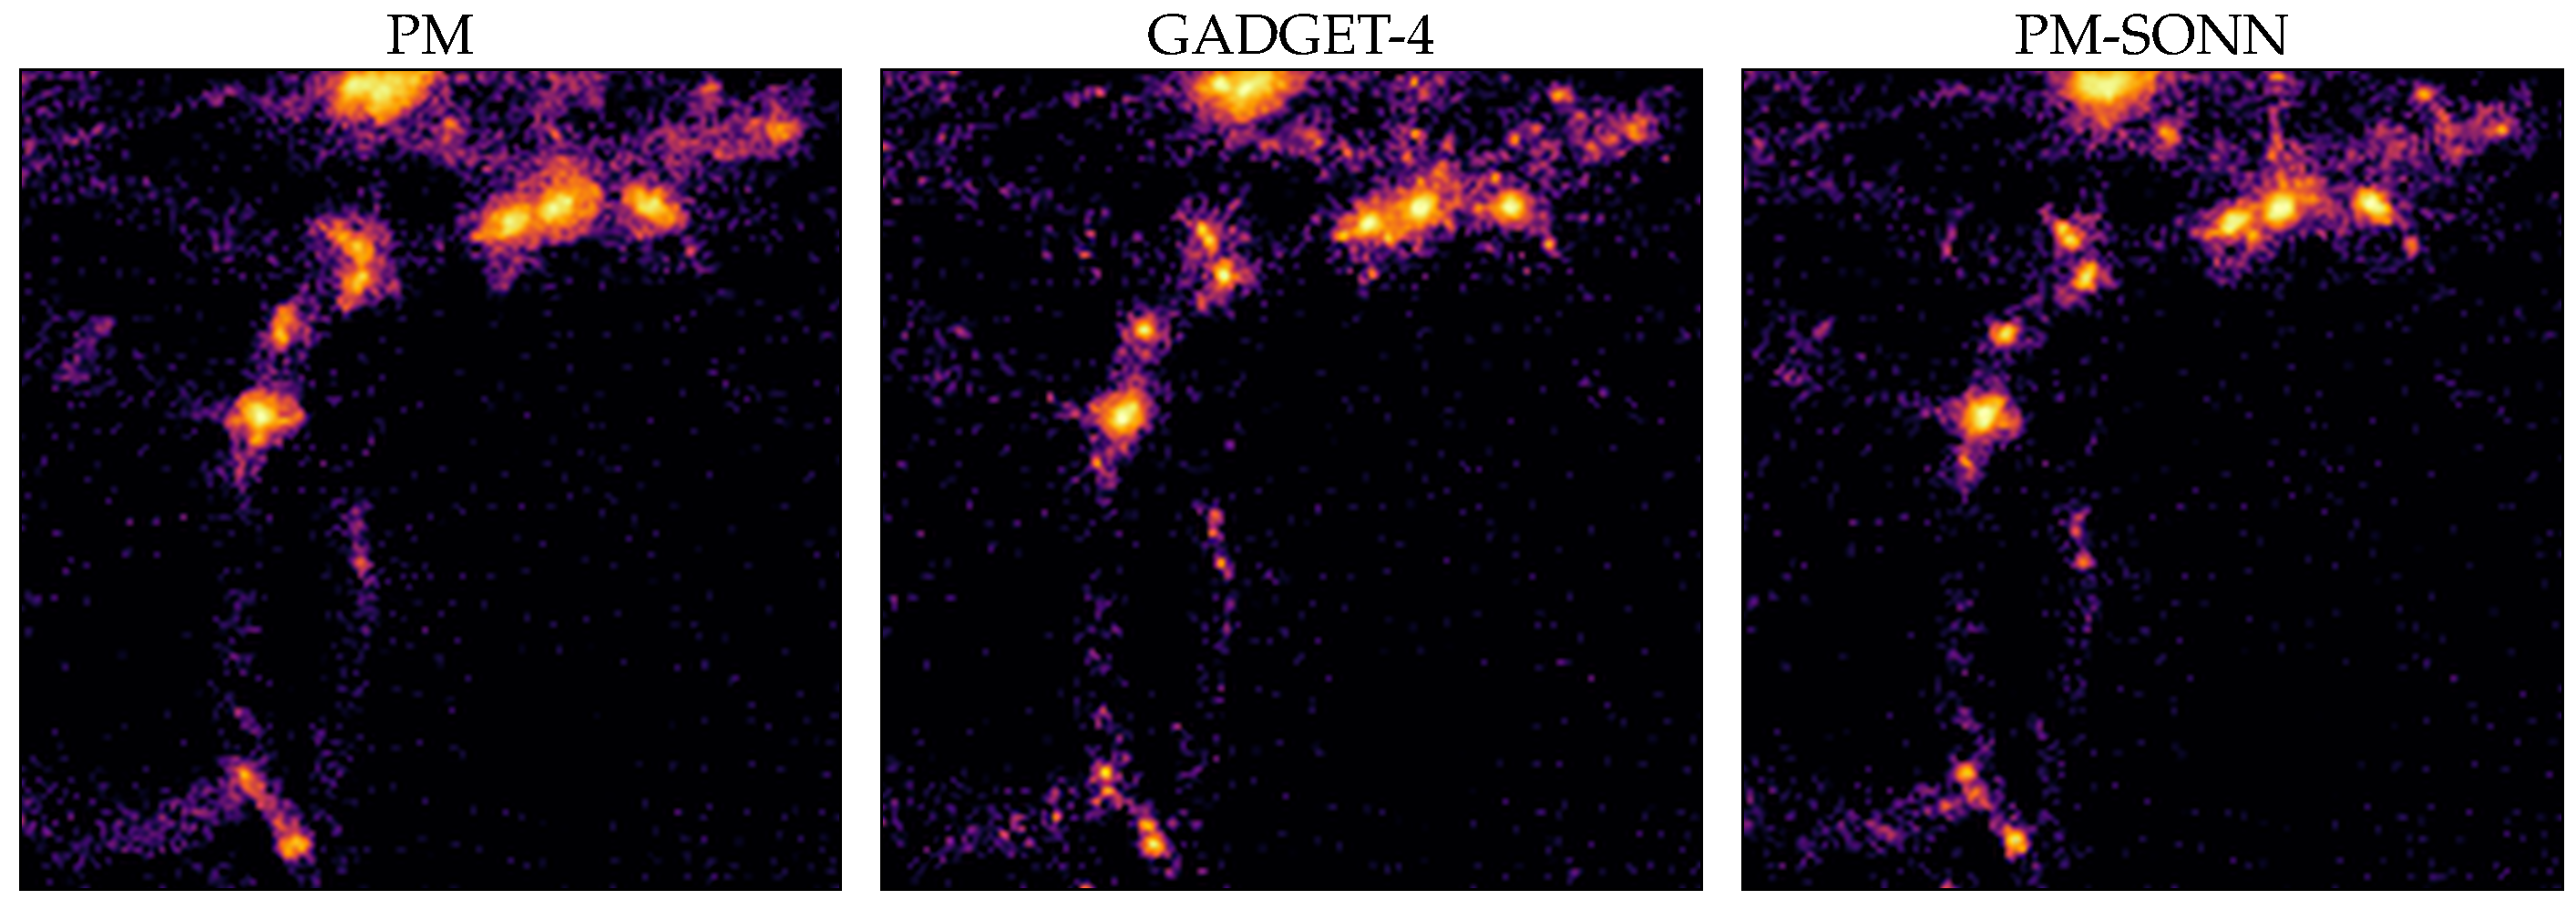
\includegraphics[width=.98\columnwidth]{slab_s0_snap120_3177874_e3000.pdf}
  \caption{Projected dark matter density fields of \GADGET\
  (\textit{middle}), original PM (\textit{left}), and optimized PM-SONN
  (\textit{right}).
  The examples here are shown for the 0th data point in our samples of
  configurations and cosmological parameters.
  This corresponds to an overall simulation box size of 79 Mpc$/h$.
  We show a zoom-in view with window length XXX Mpc$/h$, and a projected
  slab thickness of XXX Mpc$/h$.}
  \label{fig:denslab}
\end{figure*}

\begin{figure*}
  \centering
  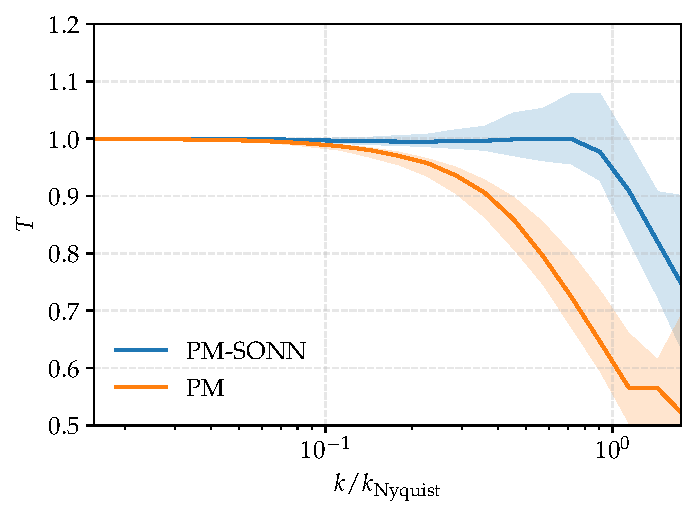
\includegraphics[width=.48\columnwidth]{tf_snap120_3177874_e3000_mid-per.pdf}
  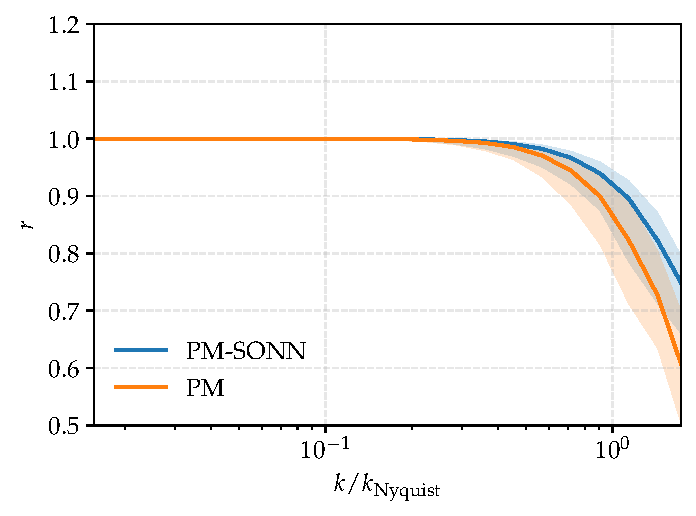
\includegraphics[width=.48\columnwidth]{cc_snap120_3177874_e3000_mid-per.pdf} \\
  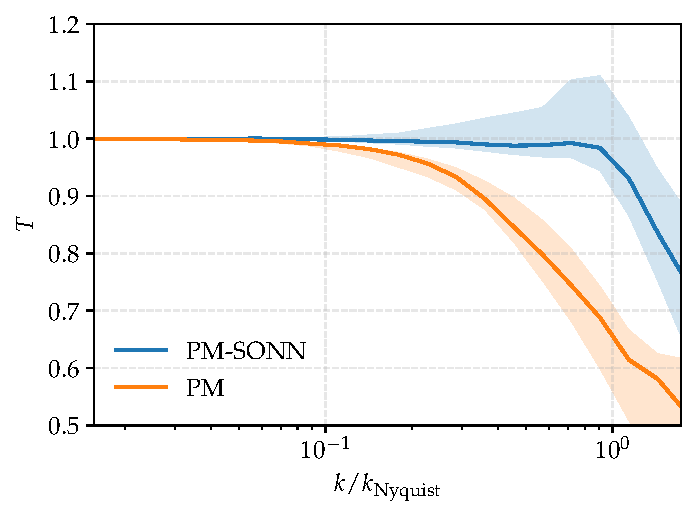
\includegraphics[width=.48\columnwidth]{tf_test_snap120_3177874_e3000_mid-per.pdf}
  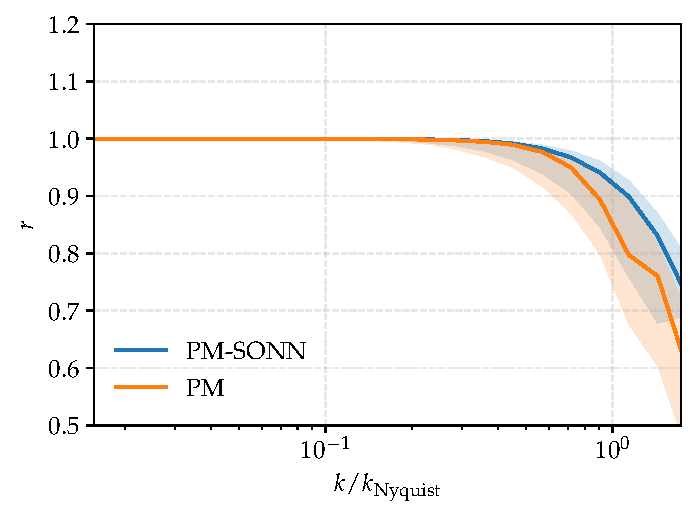
\includegraphics[width=.48\columnwidth]{cc_test_snap120_3177874_e3000_mid-per.pdf}
  \caption{The TF and CC of original PM and optimized PM-SONN simulated
  density fields with respect to that of the \GADGET.
  The solid line and shaded region indicate the median and the [16, 84]
  percentiles of different simulation configurations.
  The results are shown for the last snapshot sampled in each
  configuration, which are all around time $a\simeq 1$.
  The x-axis is the wavenumber $k$ normalized by the Nyquist wavenumber
  $k_{\rm Nyquist}$ of the particle grid, which is therefore the same
  for different box sizes.
  \textit{Upper}: results for the training dataset.
  \textit{Lower}: results for the test dataset.
  }
  \label{fig:tfcc}
\end{figure*}

As discussed in \autoref{sec:intro}, our main motivation on performing
SO of the PM method is to improve its accuracy on simulating dark matter
distribution on small scales.

The effect of SO can be visually shown by looking directly at the
density field (\autoref{fig:denslab}) on small scales.
We construct the dark matter density fields by scattering the particles
onto another mesh.
Compared to orginal PM, optimized PM with SONN is more similar to
\GADGET\ with sharper big halos and more small-scale structures.

To compare two fields $\hat f$ and $f$, we introduce for each mode the
transfer function (TF), which is defined as the square root ratio of the
auto power spectrum:
%
\begin{equation}
T(\vk) \triangleq
\sqrt{\frac{|\hat f(\vk)|^2}{|f(\vk)|^2}},
\label{T}
\end{equation}
%
and the correlation coefficient (CC):
%
\begin{equation}
r(\vk) \triangleq
\frac{\Re \bigl[ \hat f(\vk) f^*(\vk) \bigr]}
     {\sqrt{|\hat f(\vk)|^2 |f(\vk)|^2}},
\label{r}
\end{equation}
%
where the numerator is the real part of the cross power spectrum.
The two fields are identical when both $T$ and $r$ are unity.

In \autoref{fig:tfcc}, we show the results of TF and CC for both
training and test data samples.
With discrete Fourier transform (DFT) on a regular grid of length $N_c$
and cell size $l_c$, the range of sampled 1D discrete wavenumbers is
limited by the fundamental and Nyquist values, i.e. $k_{\rm fund} =
2\pi/(l_c N_c)$ and $k_{\rm Nyquist} = \pi/l_c$, where $l_c N_c$ is
simply the box size.
To show different box sizes, we normalize the wavenumber by the Nyquist
value $k_{\rm Nyquist} = \pi / l_c$ of the force mesh grid, where
$l_c$ is the cell size.
Then the normzalized wavenumber $k/k_{\rm Nyquist}$ gives the same range
$[2/N_c, 1]$ for different box sizes.
For the 3D wavenumber $k=\sqrt{\sum_{i=1}^{3}k_i^2}$, the maximum
normalized value is then $\sqrt{3}$.
The original PM method is accurate on scales much larger than the mesh
cell size, therefore $T$ and $r$ are already very close to one without
the application of SONN.
Compared to original PM, the TF of PM-SONN is improved to be consistent
with \GADGET\ within 10\% up to the particle grid Nyquist wavenumber.


\subsection{Optimized Dark Matter Halo Distributions}


\subsection{Neural Networks and Symbolic Expressions}

\begin{figure*}
  \centering
  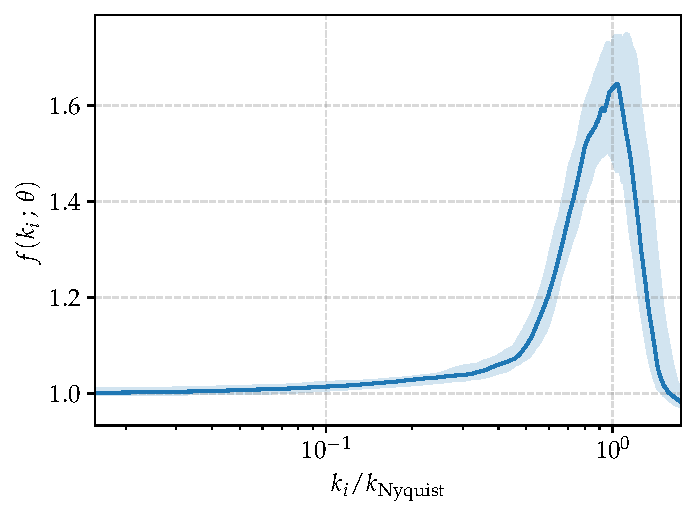
\includegraphics[width=.48\columnwidth]{net_f_a1_j3177874_e3000.pdf}
  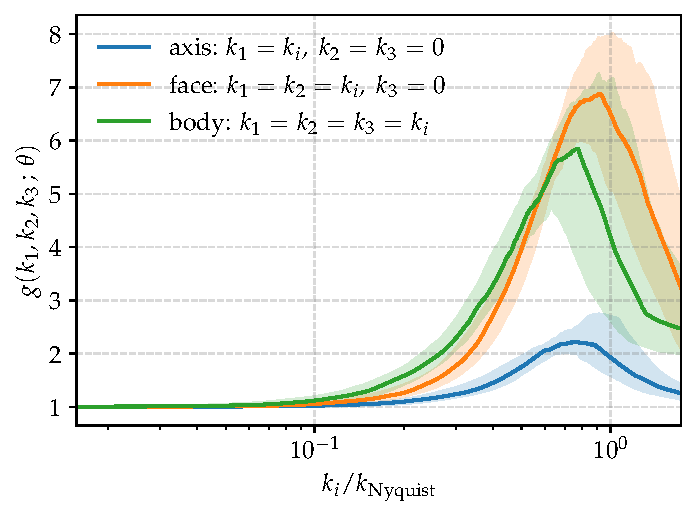
\includegraphics[width=.48\columnwidth]{net_g_a1_j3177874_e3000.pdf}
  \caption{$f(k_i; \vvartheta)$ and $g(k_1, k_2, k_3; \vvartheta)$
  functions. The solid line and shaded region indicate the median and
  the [16, 84] percentiles of the 64 sampled configurations and
  cosmological parameters. $a=1$,
  mesh shape=1}
  \label{fig:func}
\end{figure*}

For $g(k_1,k_2,k_3;\vvartheta)$, which is permutationally symmetric
about $(k_1, k_2, k_3)$, we show it as a function of the wavevector
along axis, face, and body diagonal directions.


To make the SO more interpretable and applicable to other simulations,
we fit the trained NNs with SR for analytic expressions of the $f(k_i;
\vvartheta)$ and $g(k_1, k_2, k_3; \vvartheta)$ functions.

The data for SR fitting is generated from the trained NNs, while the
input features for SR could be different from those of the NNs.
Based on the NN input features, we could further design other features
for SR fitting.

We design the input features of the NNs and SR in a way such that they
could properly fit and interpolate given our wide coverage of the
configurations and cosmological parameters.
Given the difference between NNs and SR, we could have different input
features for the two.
When generating the data for SR with the trained NNs, we could reduce or
add more features based on the existing features, with the output
unchanged.


\subsection{Benchmarks}
We compare the computational cost of \GADGET, original PM, PM-SONN, and
PM-SOSR.
In the generation of our training data, on average each \GADGET\
simulation takes about 2,000 CPU hours.


The forward evaluation of the NNs is more computation and memory
expensive compared to the analytic expressions.
We time the computation of SO for one step using NNs and SR
respectively, both after the just-in-time (JIT) compilation function
transformation in JAX.


\vspace{1em}
\section{Discussion}
% Discussion does not contain subheadings


\vspace{1em}
\section{Methods}


\vspace{1em}
\subsection{Differentiable Simulation with Observables}
\label{sec:diffsim_obs}

\begin{figure*}[t]
\centering
\tikzstyle{node style}=[
  node distance=2.8em, minimum size=2.8em, text centered,
  integ/.style={to-, gray, thick},
  obs/.style={to-, gray, thick, dashed},
  from/.style={to-, gray, thick, dotted},
]
\tikzstyle{box style}=[
  rectangle, inner sep=0.4em, rounded corners, draw=gray, thick,
]
\subfloat[integration-observation loop]{
\label{fig:loop}
\begin{tikzpicture}[node style]
  \node (z_0) {$\vz_0$};
  \node (o_0) [below=of z_0] {$\vo_0$}
        edge [obs] (z_0);
  \node (z_0i) [right=of z_0] {$\cdots$}
        edge [integ] (z_0);
  \node (o_1i) [below=of z_0i] {$\cdots$}
        edge [obs] (z_0i)
        edge [from] (o_0);
  \node (z_i) [right=of z_0i] {$\vz_i$}
        edge [integ] (z_0i);
  \node (o_i) [below=of z_i] {$\vo_i$}
        edge [obs] (z_i)
        edge [from] (o_1i);
  \node (z_in) [right=of z_i] {$\cdots$}
        edge [integ] (z_i);
  \node (o_in) [below=of z_in] {$\cdots$}
        edge [obs] (z_in)
        edge [from] (o_i);
  \node (z_n) [right=of z_in] {$\vz_n$}
        edge [integ] (z_in);
  \node (o_n) [below=of z_n] {$\vo_n$}
        edge [obs] (z_n)
        edge [from] (o_in);
  \node (obj) [right=of o_n] {$\cJ$}
        edge [from] (o_n);
  \node (box) [box style, fit=(z_0) (o_n)] {};
  \useasboundingbox ($ (box.south) - (0, 1em) $) --
                    ($ (box.north) + (0, 1em) $);
\end{tikzpicture}
}
\\
\subfloat[leapfrog integration-observation step]{
\label{fig:step}
\begin{tikzpicture}[node style]
  \node (z_left) [minimum height=3.5em] {};
  \node (o_left) [below=of z_left] {};
  \node (z_0) [minimum height=3.5em, right=of z_left]
        {$\begin{pmatrix} \vx_{i-1} \\ \vp_{i-1} \end{pmatrix}$}
        edge [integ] (z_left);
  \node (o_0) [below=of z_0] {$\vo_{i-1}$}
        edge [obs] (z_0)
        edge [from] (o_left);
  \node (z_01) [minimum height=3.5em, right=of z_0]
        {$\begin{pmatrix} \vx_{i-1} \\ \vp_{i-\half} \end{pmatrix}$}
        edge [integ] node[below] {Kick} (z_0);
  \node (z_02) [minimum height=3.5em, right=of z_01]
        {$\begin{pmatrix} \vx_i \\ \vp_{i-\half} \end{pmatrix}$}
        edge [integ] node[below] {Drift} (z_01);
  \node (z_1) [minimum height=3.5em, right=of z_02]
        {$\begin{pmatrix} \vx_i \\ \vp_i \end{pmatrix}$}
        edge [integ] node[below] {Kick} (z_02);
  \node (o_1) [below=of z_1] {$\vo_i$}
        edge [obs] (z_1)
        edge [from] (o_0);
  \node (z_right) [minimum height=3.5em, right=of z_1] {}
        edge [integ] (z_1);
  \node (o_right) [right=of o_1] {}
        edge [from] (o_1);
  \useasboundingbox ($ (box.south) - (0, 1em) $) --
                    ($ (box.north) + (0, 1em) $);
\end{tikzpicture}
}
\caption{Forward simulation with observables.
\subref{fig:loop} shows the flow of the state $\vz$ and the
observable $\vo$ in the integration-observation loop of the forward
simulation.
\subref{fig:step} shows explicitly one integration-observation step for
the leapfrog integrator.
The solid lines denote the integration of the state, the dashed lines
denote the observation of the state added to the observable, and the
dotted lines are simply the forward pass of the previous observable.}
\end{figure*}

The gradient descent optimization of the neural networks embedded in the
Poisson equation \eqref{force_so} relies on the backpropagation of the
gradients throughout the simulation.
In this work, we use the PM $N$-body library \pmwd\ \citep{Li2022b},
which is an implementation of the differentiable cosmological simulation
with the adjoint method \citep{Li2022a}.

Here we extend the original framework with a more detailed
implementation of observables that is explicitly formulated for this
work.
Following \cite{Li2022a}, we denote the particles' state with $\vz =
(\vx, \vp)^\intercal$, where $\vx$ and $\vp$ are the positions and
momenta of the particles.
For the forward simulation (\autoref{fig:loop}), we consider the
evolution of the observable $\vo$ along with the state $\vz$ following
\begin{align}
\vz_i &= \vz_{i-1} + \vI_{i-1}(\vz_{i-1}, \vtheta), \\
\vo_i &= \vo_{i-1} + \vO_i(\vz_i, \vtheta), \qquad i=1,\cdots,n
\label{IO_fwd}
\end{align}
where $\vI$ and $\vO$ are the integration and observation functions
respectively, and we observe the new state every step after it is
updated from the integration function.
The observable is initialized by observing the initial state
\begin{equation}
\vo_0 = \vO_0(\vz_0, \vtheta).
\label{O_init}
\end{equation}
Notice that we take an observation function $\vO$ that depends only on
the state but not the observable itself, which is consistent with the
case in this work where the observable includes multiple snapshots at
different times and therefore the state of particles at each step
contributes independently to the observable, as discussed in
\autoref{sec:snapobs}.
The derivation below remains much the same with minor modifications for
a more general observation function.

Now we derive the adjoint equations with observables.
Assuming an objective function of the observable at the final time step,
the Lagrangian reads
\begin{align}
\cL = \cJ(\vo_n)
&- \sum_{i=1}^{n} \vlambda_i
  \cdot \bigl[ \vz_i - \vz_{i-1} - \vI_{i-1}(\vz_{i-1}, \vtheta) \bigr] \nonumber\\
&- \sum_{i=1}^{n} \vmu_i
  \cdot \bigl[ \vo_i - \vo_{i-1} - \vO_i(\vz_i, \vtheta) \bigr],
\label{IO_Lagrangian}
\end{align}
where the multipliers $\vlambda$ and $\vmu$ are the adjoint variables of
$\vz$ and $\vo$ respectively.
Taking the full derivative of $\cL$ with respect to $\vtheta$ and
collecting the terms with $\p\vz_i/\p\vtheta$ and $\p\vo_i/\p\vtheta$,
the adjoint equations arise as
\begin{align}
\vmu_{i-1} &= \vmu_i, \\
\vlambda_{i-1} &= \vlambda_i
  + \vlambda_i\cdot\frac{\p\vI_{i-1}}{\p\vz_{i-1}}
  + \vmu_{i-1}\cdot\frac{\p\vO_{i-1}}{\p\vz_{i-1}}, \qquad i=n,\cdots,1
\label{IO_adj}
\end{align}
with the initial conditions
\begin{equation}
\vmu_n = \frac{\p\cJ}{\p\vo_n},\
\vlambda_n = \vmu_n\cdot\frac{\p\vO_n}{\p\vz_n}.
\label{IO_adj_init}
\end{equation}
The simple constant backpropagation of $\vmu$ results from the form of
the forward modeling, where neither the integration nor the observation
function depends on the observable.
The initial condition of the observable \eqref{O_init} gives
\begin{equation}
\frac{\p\vo_0}{\p\vtheta} = \frac{\p\vO_0}{\p\vtheta}
+ \frac{\p\vO_0}{\p\vz_0}\cdot\frac{\p\vz_0}{\p\vtheta},
\end{equation}
which could be substituted into the full derivative for further
simplification.
Finally, the objective gradients could be accumulated through
\begin{align}
\frac{d\cJ}{d\vtheta} =
\vlambda_0\cdot\frac{\p\vz_0}{\p\vtheta}
+ \sum_{i=1}^{n} \left[\vlambda_i\cdot\frac{\p\vI_{i-1}}{\p\vtheta}
+ \vmu_{i-1}\cdot\frac{\p\vO_{i-1}}{\p\vtheta}\right]
+ \vmu_{n}\cdot\frac{\p\vO_{n}}{\p\vtheta},
\label{IO_grad}
\end{align}
where the terms are organized to be consistent with the adjoint
equations.

With the particles' state $\vz = (\vx, \vp)^\intercal$ updated with the
leapfrog integrator (\autoref{fig:step}), each integration-observation
step could be explicitly expanded as
\begin{align}
\vp_{i-\half} &= \vp_{i-1} + \va_{i-1} K(t_{i-1}, t_{i-1}, t_{i-\half}), \nonumber\\
\vx_i &= \vx_{i-1} + \vp_{i-\half} D(t_{i-\half}, t_{i-1}, t_i), \nonumber\\
\vp_i &= \vp_{i-\half} + \va_i K(t_i, t_{i-\half}, t_i), \nonumber\\
\vo_i &= \vo_{i-1} + \vO_i(\vx_i, \vp_i),
\label{KDKO}
\end{align}
where $K$ and $D$ are the kick and drift operators \citep{Li2022a}, and
the acceleration is computed with force evaluation as
\begin{equation}
\va_i \triangleq -\vnabla\varphi(\vx_i).
\end{equation}
Now the explicit adjoint equations with observables for the leapfrog
integrator follows
\begin{align}
\vmu_{i-1} &= \vmu_i, \nonumber\\
\vxi_{i-\half} &= \vxi_i + \vpi_i \cdot \frac{\p\va_i}{\p\vx_i} K(t_i, t_i, t_{i-\half}), \nonumber\\
\tilde{\vpi}_{i-1} &= \vpi_i - \vxi_{i-\half} D(t_{i-\half}, t_i, t_{i-1}), \nonumber\\
\tilde{\vxi}_{i-1} &= \vxi_{i-\half} + \tilde{\vpi}_{i-1} \cdot \frac{\p\va_{i-1}}{\p\vx_{i-1}} K(t_{i-1}, t_{i-\half}, t_{i-1}), \nonumber\\
\vxi_{i-1} &= \tilde{\vxi}_{i-1} + \vmu_{i-1}\cdot\frac{\p\vO_{i-1}}{\p\vx_{i-1}}, \nonumber\\
\vpi_{i-1} &= \tilde{\vpi}_{i-1} + \vmu_{i-1}\cdot\frac{\p\vO_{i-1}}{\p\vp_{i-1}},
\label{KDKO_adj}
\end{align}
with initial conditions
\begin{equation}
\vmu_n = \frac{\p\cJ}{\p\vo_n},\
\vxi_n = \vmu_n \cdot \frac{\p\vO_n}{\p\vx_n},\
\vpi_n = \vmu_n \cdot \frac{\p\vO_n}{\p\vp_n}.
\label{KDKO_adj_init}
\end{equation}
The objective gradients now reads
\begin{align}
\frac{\d\cJ}{\d\vtheta} =\
& \vxi_0 \cdot \frac{\p\vx_0}{\p\vtheta}
+ \vpi_0 \cdot \frac{\p\vp_0}{\p\vtheta}
+ \vmu_{n}\cdot\frac{\p\vO_{n}}{\p\vtheta} \nonumber\\
& - \sum_{i=1}^n \Bigl[
  \vpi_i\cdot\bigl(\va_i \frac\p{\p\vtheta} + \frac{\p\va_i}{\p\vtheta}
    \bigr) K(t_i, t_i, t_{i-\half}) \nonumber\\
  &\qquad + \vxi_{i-\half} \cdot \vp_{i-\half}
    \frac{\p D(t_{i-\half}, t_i, t_{i-1})}{\p\vtheta} \nonumber\\
  &\qquad + \tilde{\vpi}_{i-1}\cdot\bigl(\va_{i-1} \frac\p{\p\vtheta}
    + \frac{\p\va_{i-1}}{\p\vtheta} \bigr) K(t_{i-1}, t_{i-\half}, t_{i-1}) \nonumber\\
  &\qquad + \vmu_{i-1}\cdot\frac{\p\vO_{i-1}}{\p\vtheta}
\Bigr].
\label{KDKO_grad}
\end{align}
The backward evolution of the adjoint variables is carried out along
with the reverse-time integration of the particles' state following
exactly the same path of the forward integration, which is necessary to
get the primals for the evaluation of the Jacobians.


\vspace{1em}
\subsection{Observation of Snapshots with Interpolation}
\label{sec:snapobs}

The $N$-body time integration is carried out along discrete time steps
in terms of the scale factor $a$, and the state of particles at any
given time can be achieved using interpolation.
Given the particle displacements $\vs$ and velocities\footnote{The
velocity is related to the canonical momentum $\vp$ through $\vv =
\vp/(a^3H)$, where $H$ is the Hubble parameter.} $\vv \triangleq
\d\vs/\d a$ at two consecutive time steps $a_i$ and $a_{i+1}$, we get
the snapshot of particles in between at $a$ using the cubic Hermite
interpolation.
The interpolated particle displacements are given by
\begin{align}
  \vs(a) =\ &h_{00}(\alpha)\vs_i + h_{10}(\alpha)(a_{i+1} - a_i)\vv_i + \nonumber\\
           &h_{01}(\alpha)\vs_{i+1} + h_{11}(\alpha)(a_{i+1} - a_i)\vv_{i+1},
\end{align}
where $\alpha \triangleq (a - a_i)/(a_{i+1} - a_i)$ and the Hermite
basis functions read
\begin{align}
  h_{00}(\alpha) &= 2\alpha^3 - 3\alpha^2 + 1, \nonumber\\
  h_{10}(\alpha) &= \alpha^3 - 2\alpha^2 + \alpha, \nonumber\\
  h_{01}(\alpha) &= -2\alpha^3 + 3\alpha^2, \nonumber\\
  h_{11}(\alpha) &= \alpha^3 - \alpha^2.
\end{align}
The particle velocities are then given by the derivative $\vv(a) =
\d\vs(a) / \d a$.
Notice that the cubic Hermite interpolation is a linear combination of
the particles' states at two consecutive time steps and each state
contributes independently to the interpolated snapshot, which is
consistent with our formulation in \eqref{IO_fwd} where the
observation function does not depend on the observable from the previous
step.
The coefficients are the only difference between the first and second
half of the interpolation.
A series of interpolated snapshots at given times constitute our
observable for the objective function.
Therefore for the observation at each step, we first determine if the
current particles' state contributes to any of the interpolated
snapshots in observable.
If it does, we then perform the interpolation depending on whether it
is the first or the second half, and finally add this update to the
corresponding snapshot in observable.


\vspace{1em}
\subsection{Training Data and Configurations}

\begin{figure*}
  \centering
  
\includegraphics[width=0.9\linewidth]{sobol.pdf}
  \caption{Randomized Quasi-Monte Carlo (RQMC) configuration with
    scrambled Sobol sequence of 512 points in 9D.
    Lower triangular panels show the 2D projections and the diagonal
    panels are the 1D cumulative histograms.
    From left to right (top to bottom), we use each dimension of the
    sample to scale the parameters as ordered in \autoref{tab:param}.
    We use the \texttt{scipy.stats.qmc} package \citep{SciPy} to
    generate the Sobol sequence \citep{Sobol1967}, which uses the
    direction number from \citet{JoeKuo2008} and the Owen scrambling
    \citep{Owen1998}.
    We search among 65536 scrambling seeds to minimize the mixture
    discrepancy (a uniformity measure) proposed in \citet{Zhou2013MD}.
  }
  \label{fig:sobol}
\end{figure*}

We configure \GADGET\ with high force and time integration accuracy
settings.
For gravitational force, we choose pure FMM with $p=5$ and opening angle
0.4.
%FIXME list other from Config.sh and param.txt

We sample 512 data points in the 9D space of configurations and
cosmological parameters using randomized quasi-Monte Carlo (RQMC) method
with scrambled Sobol sequence (\autoref{fig:sobol}).
We use the \texttt{scipy.stats.qmc} package \citep{SciPy} to generate
the Sobol sequence \citep{Sobol1967}, which uses the direction number
from \citet{JoeKuo2008} and the Owen scrambling \citep{Owen1998}.
We search among 65536 scrambling seeds to minimize the mixture
discrepancy (a uniformity measure) proposed in \citet{Zhou2013MD}.

In addition, we sample 9 extra data points for the interpolation test of
the trained model to different configurations and cosmological
parameters.

Small numerical differences in initial conditions (ICs) could become
more significant with the $N$-body evolution.
Therefore, besides the output snapthos, the ICs used in the \GADGET\
simulations are also loaded from file during training to make sure the
ICs are consistent for both the training data and the \pmwd\ model.


\vspace{1em}
\subsection{Physical Features}
\label{sec:features}

\begin{table}
  \centering
  \caption{Possible features that can affect force sharpening, detailed
  in \autoref{sec:features}. Scales could be multiplied by the
  wavenumber $k$ to form dimensionless factors.}
  \label{tab:feat}
  \begin{tabular}{rl}
  \toprule
  type & feature \\
  \midrule
  & $R_\mathrm{d}$: RMS linear displacement \\
  \cmidrule(lr){2-2}
  & $R_P$: $\Delta_\linear^2(R_P^{-1}) \triangleq 1$ \\
  \cmidrule(lr){2-2}
  nonlinear scales & $R_\tophat$: $\sigma_\tophat^2(R_\tophat) \triangleq 1$ \\
  \cmidrule(lr){2-2}
  & $R_\gauss$: $\sigma_\gauss^2(R_\gauss) \triangleq 1$ \\
  \cmidrule(lr){2-2}
  & $\d R / \d\lna$: time derivatives of the above \\
  \midrule
  & $l_p$: particle spacing \\
  \cmidrule(lr){2-2}
  other scales & $l_c$: PM force mesh cell size \\
  \cmidrule(lr){2-2}
  & $l_s$: softening length \\
  \midrule
  & $G_m(a) \triangleq D_m(a) / a^m, m \in \{1, 2, \YL{3's?}\}$ \\
  \cmidrule(lr){2-2}
  & $\d\ln G_m / \d\lna$ \\
  \cmidrule(lr){2-2}
  dimensionless factors & $\Omegam(a), \YL{\OmegaK(a)}$ \\
  \cmidrule(lr){2-2}
  & $\d\ln\!H / \d\lna$ \\
  \cmidrule(lr){2-2}
  & $\Delta\lna$: time step size in $\lna$ \\
  & \YL{Now this can be an important feature with varying $a_\ic$} \\
  \bottomrule
  \end{tabular}
  \end{table}

In this section, we introduce a list of physical quantities that could
be of possible importance in SO.
These quantities are used in the input features for either the NNs or
SR.
Multiple scales and dimensionless factors could possibly affect force
sharpening.
A list of these features is summarized in \autoref{tab:feat}, and here
we present relevant definitions and more details.

Below are some definitions related to the typical spatial scales.
\begin{itemize}
\item The root-mean-square (RMS) linear displacement is given by
%
\begin{equation}
R_\mathrm{d}^2 = \int \frac{k P_\linear(k)}{6\pi^2} \d\lnk,
\end{equation}
%
where $P_\linear(k)$ is the linear power spectrum.
\item The dimensionless linear power spectrum is defined as
%
\begin{equation}
\Delta^2_\linear(k) \triangleq \frac{k^3 P_\linear(k)}{2 \pi^2},
\end{equation}
%
based on which we define a nonlinear scale $R_P$ through
$\Delta_\linear^2(R_P^{-1}) \triangleq 1$.
\item The variance of linear matter overdensity in a top-hat window is given by
%
\begin{equation}
\sigma_\tophat^2(R) = \int_0^\infty \frac{\d k}k
  \Delta_\linear^2(k) W_\tophat^2(kR),
\end{equation}
%
where $W_\tophat(kR) = 3[\sin(kR) - kR\cos(kR)] / (kR)^3$ is the
Fourier transform of the top-hat window.
Then we have $R_\tophat$ defined through $\sigma_\tophat^2(R_\tophat)
\triangleq 1$.
\item Likewise $\sigma_\gauss^2(R)$ is defined with a Gaussian window
$W_\gauss(kR) = e^{-(kR)^2/2}$, and $R_\gauss$ with
$\sigma_\gauss^2(R_\gauss) \triangleq 1$.
\end{itemize}
These nonlinear scales are functions of time since the linear power
spectrum evolves with time through the growth factor $D(a)$, we could
also take the time derivatives of these scales as possible features.
Other relevant scales include the particle spacing $l_p$ in Lagrangian
space, the cell size $l_c$ of the chosen mesh grid for force evaluation,
and the softening length $l_s$ in the target \GADGET\ simulations.

Scales could be multiplied with the wavenumber $k$ to form dimensionless
quantities.
For example, the product of $k$ with the mesh cell size $l_c$ results in
a quantity $kl_c = \pi k/k_{\rm Nyquist}$ that is invariant to different
box sizes, which should be an important feature.

Relevant scale-independent dimensionless factors are
\begin{itemize}
\item $G_m(a) \triangleq D_m(a) / a^m$: linear growth given in
  suppression factors for $m \in \{1, 2\}$;
\item $\d\ln G_m / \d\lna$: with $m=1$ case related to the growth rate
  $f \triangleq \d\ln D_1 / \d\lna$;
\item $\Omegam(a)$: matter density parameter at $a$;
\item $\d\ln\!H / \d\lna$: time derivative of Hubble expansion;
\item $\Delta\lna$: time step size in $\lna$.
\end{itemize}


\vspace{1em}
\subsection{Loss Function}
\label{sec:loss}

The loss function is constructed by comparing the simulated field $\hat
f$ with the target field $f$.
In this work, we consider two fields in our loss function, the
Lagrangian particle displacement field $\vs(\vq)$ and the Eulerian
density field $\delta(\vx)$.

For the displacement field, the mean squared error (MSE) loss has been
proved effective in many previous works
\citep[e.g.,][]{HeEtAl2019, LiEtAl2021}:
%
\begin{equation}
\cL_\vs = \ln \frac{\sum_\vq \bigl\lfloor \hat\vs(\vq) - \vs(\vq) \bigr\rceil^2}
                   {\sum_{\vq'} s(\vq')^2},
\end{equation}
%
in which a particle originating from its Lagrangian position $\vq$ is
displaced by $\vs$ in the \GADGET\ snapshot and by $\hat\vs$ in the
prediction of \pmwd\ model in training.
$\lfloor\rceil$ rounds the residual displacements to the range between
negative to positive half box size, accounting for the periodic
boundaries important for the smallest boxes in \autoref{tab:param}.
Note that we have further taken the logarithm to combine it with the
other loss(es).
Even though the logarithm should be enough for adaptive optimizer and
fixed simulation configuration, this may create problem in our training
on all configurations at the same time.
So normalizations inside the logarithm is added above and below.
% Say that only s loss is not enough even though in principle it is,
% and cite DrewEtAl x2 too

However, for the density field in the Eulerian space, an MSE loss is
dominated by the small scale modes.
In this work we choose uniform weights in the scale space on the
relative MSE.
We bin the modes logarithmically by \nicefrac13 octave in scale, with
the $i$-th $k$-bin $K_i \triangleq [k_i, k_{i+1})$, where $k_i =
2^{1+i/3} \pi / L$.
We introduce a loss function that sums up its MSE relative to the target
field power in logarithmic bins:
%
\begin{equation}
  \cL_\delta = \frac1{N_K} \sum_i \ln \biggl[
  \frac{\sum_{\vk \in K_i} \bigl| \hat \delta(\vk) - \delta(\vk) \bigr|^2}
       {\sum_{\vk' \in K_i} | \delta(\vk')|^2} + \epsilon \biggr],
\label{loss_power_ln}
\end{equation}
%
where $N_K$ is the number of $k$-bins, and $\epsilon$ sets the relative
threshold tolerance, below which we consider $\hat \delta$ in each $K$
accurate enough and the gradients from that bin less important.

% Under the mild assumptions that $T$ \eqref{T} and $r$ \eqref{r} are smooth
% and isotropic, we can show
% %
% \begin{equation}
% \cL_\delta \propto \int \!\d\ln\!k\, \ln
% \Bigl\{ \bigl[ 1 - T(\vk) \bigr]^2
%   + 2 T(\vk) \bigl[ 1 - r(\vk) \bigr] \Bigr\} \geq -\infty,
% \end{equation}
% %
% replacing
% %
% \begin{equation}
% \cL_\delta \propto \int \!\d\ln\!k\, w(\vk)
% \Bigl\{ \bigl[ 1 - T(\vk) \bigr]^2
%   + 2 T(\vk) \bigl[ 1 - r(\vk) \bigr] \Bigr\} \geq 0,
% \end{equation}
% %
% that only vanishes when both $T$ and $r$ are unity for all modes, i.e.,
% when $\hat\delta$ is identical to $\delta$.
% Above we choose the binned version instead for the robustness against
% the noisy modewise $|\delta(\vk)|^2$ in the denominator.
% The derivation here is similar to that in \citet{HeEtAl2019} on the MSE
% loss, while our modification is important to balance among all scales so
% that the neural network does not focus too much on either high or low
% $k$'s.

We combine the two fields to form the total loss for a single snapshot,
and further sum over all snapshots in a single forward simulation
%
\begin{equation}
\cJ = \sum_{a_i} \left[\cL_{\vs(a_i)} + \cL_{\delta(a_i)}\right].
\end{equation}
%


\vspace{1em}
\subsection{Training of Neural Networks}

We initialize the parameters of NNs in a way such that the output is
around one with slight deviations, i.e. roughly the original PM without
SO.
This is achieved by setting the kernel of the output layer to be very
small random values and the bias to be zero, whose return is then around
one after the exponential function.
The parameters are initialized to be the same for all devices, and hence
remain the same during training given the same averaged gradients.

We perform distributed data-parallel training using GPU devices hosted
across multiple computing nodes.
With data parallelism, the training data samples are uniformly
distributed to the processes with each process binded to a single GPU
device.
In total, we use 16 \GPU\ GPUs, each accompanied with 8 CPU cores
and 125 GB CPU memory mainly for preloading the training data.
The order of data samples within each process is shuffled across
training epochs.
In each training step, a data sample is fed into the GPU from the CPU
memory where the preloading took place to save the repeated reading time
from the disk.

For each training step, we configure and run \pmwd\ with the same
initial coniditions, cosmological parameters and other common
configurations as the training data sample.
As discussed in \autoref{sec:loss}, the loss in a single simulation sums
over all snapshots.
Our batch size is 16, i.e. the number of GPU devices, since one
simulation is run on a single GPU and compared to the corresponding
training data sample for loss.
The loss and gradients are collected and averaged across all GPU
devices, with which the optimizer is updated.
We use the Adam \citep{Adam} optimizer.

% We use Optuna \citep{optuna_2019} to search for the optimal
% hyperparameters.

% We empoly a learning rate scheduler that reduces the learning rate on
% plateau where the loss function stops decreasing.
% The initial learning rate is set at [...] with a reduction factor of
% [...] after [...] epochs of no decreasing on loss.

Same as the \pmwd\ library, this work is also implemented using JAX
\citep{JAX}.
We implement the NNs with \texttt{Flax} \citep{flax2020github}, and use
the optimizers provided in \texttt{Optax}, part of the DeepMind JAX
Ecosystem \citep{deepmind2020jax}.


\vspace{1em}
\subsection{Sensitivity Analysis}
\label{sec:sensitivity}
For the trained $f(k_i; \vvartheta)$ and $g(\vk; \vvartheta)$ neural
networks, we perform the derivative-based global sensitivity measure
(DGSM) to analyze their dependence on the configuration and cosmological
parameters $\vvartheta$ sampled with the Sobol sequence as shown in
\autoref{tab:param}.

For each sample $\vvartheta^{(i)}$, we compute the gradient of the neural
network, $\partial f / \partial \vvartheta^{(i)}$.
The importance sensitivity index $\vnu$ is then computed as the mean
squared gradient, normalized by both the input and output variances to
account for different parameter scales and to enable comparison across
outputs:
\begin{equation}
\vnu = \frac{\mathrm{Var}(\vvartheta)}{\mathrm{Var}(f)} \frac{1}{N} \sum_{i=1}^{N}
  \left(\frac{\partial f}{\partial \vvartheta^{(i)}}\right)^2,
\end{equation}
where $\vnu$ and $\mathrm{Var}(\vvartheta)$ are of the same shape as $\vvartheta$,
and $\mathrm{Var}(f)$ is a scalar.

An alternative formulation uses the elasticity, defined as
\begin{equation}
\varepsilon \triangleq \frac{\partial f}{\partial \vvartheta} \cdot \frac{\vvartheta}{f}
= \frac{\partial \ln f}{\partial \ln \vvartheta},
\end{equation}
which measures the percentage change in output per percentage change in input.
The elasticity-based sensitivity index is then computed as the mean squared
elasticity
\begin{equation}
\vnu_\varepsilon = \frac{1}{N} \sum_{i=1}^{N} \varepsilon^{(i)2},
\end{equation}
where the normalization by $\vvartheta^2/f^2$ is applied per sample before
averaging. This provides a scale-invariant measure that is particularly useful
when comparing sensitivities across parameters with different units or orders
of magnitude.


\vspace{1em}
\subsection{Symbolic Regression Fitting}

To perform further analyses of the trained NNs, including feature
importance analysis and symbolic regression fitting, we need to generate
samples of (input, output) data.
The input features of the NNs are constructed based on the RQMC
parameters in \autoref{tab:param}, the wavenumber $k$, and the scale
factor $a$.
Again, we use Sobol sequence to sample data points in this high
dimensional space.

We use the random forest regressor for feature selection using
impurity-based importance.
We use the \texttt{scikit-learn} \citep{scikit-learn} code for this.
% more details on the hyperparams in random forest
\YZ{Maybe we can add another column in \autoref{tab:feat} for feature
importance?}

The selected important features are then used for SR.
We use the \texttt{PySR} \citep{PySR} SR code to fit for analytic
function expressions of the trained SO neural networks.

\YL{It is interesting to symbolically regress $f$, $k_i f$, and $f g$
etc to see which one gives simpler expression, given the possible
different rankings by complexity.
For example, $k_i f(k_i)$ may have a simpler form as a nonlinear odd
function.}


\vspace{1em}
\textit{\large Acknowledgements:}
We thank Qiufan Lin, Paulo Montero-Camacho, and Yang Wang for helpful
discussions.
YZ and YL are supported by The Major Key Project of PCL.
YZ is supported by the National Natural Science Foundation of China
under Grant No. 12503006.
YZ was also supported by the China Postdoctoral Science Foundation under
Grant No. 2023M731831.
The Flatiron Institute is supported by the Simons Foundation.


\vspace{1em}
\textit{\large Data Availability:}
We make the \GSDATA\ simulation dataset public at ...


\vspace{1em}
\textit{\large Code Availability:}
\pmwd\ \citep{Li2022b} is open-source on GitHub
\href{https://github.com/eelregit/pmwd}{\faGithub}, including the source
files and scripts of this paper
\href{https://github.com/eelregit/pmwd/tree/master/docs/papers/sto}{\faFile}.
\GADGET\ \citep{GADGET-4} can be obtained through a public
git-repository \href{http://gitlab.mpcdf.mpg.de/vrs/gadget4}{\faGitlab},
hosted by a gitlab server at the Max-Planck Computing and Data Facility
(MPCDF).



\bibliographystyle{aasjournal}
\bibliography{sto}


\vspace{1em}
\appendix
% supplementary information of Nat. Mach. Intell.


\vspace{1em}
\section{Tests on Differentiable Simulation with Observables}

\begin{figure*}
  \centering
  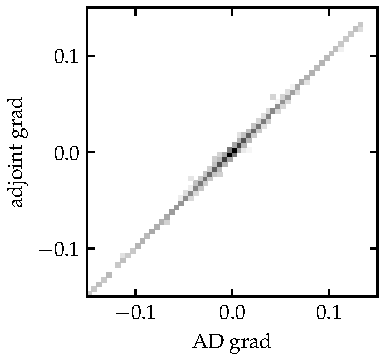
\includegraphics[width=.48\textwidth]{ptcl_grad_cmp.pdf}
  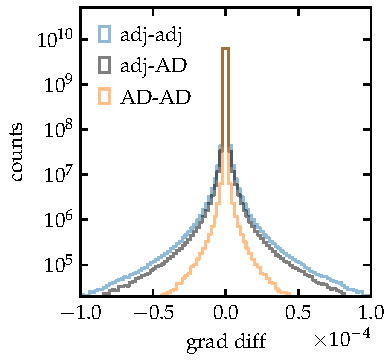
\includegraphics[width=.48\textwidth]{ptcl_grad_diff.pdf}
  \caption{Objective gradients of the initial particles' displacement of
    $N$-body integration-observation loop, i.e. $\vxi_0 = d\cJ/d\vx_0$.}
  \label{fig:ptcl_grad}
\end{figure*}

\begin{figure*}
  \centering
  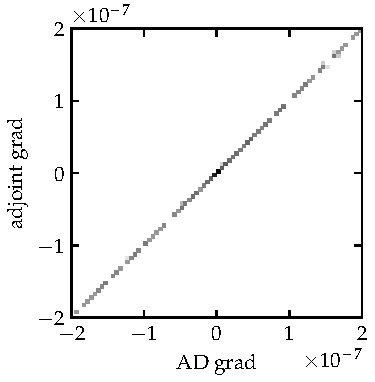
\includegraphics[width=.48\textwidth]{sonn_grad_cmp.pdf}
  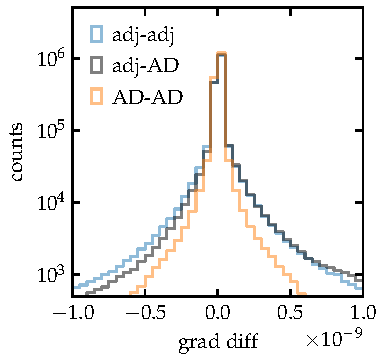
\includegraphics[width=.48\textwidth]{sonn_grad_diff.pdf}
  \caption{Objective gradients of the SO neural network parameters, i.e.
  $d\cJ/d\vtheta$.}
  \label{fig:sonn_grad}
\end{figure*}

In \autoref{sec:diffsim_obs} we derived the adjoint equations and
objective gradients in the framework of the adjoint method for the
differentiable simulation with observables.
Here we perform tests on our implementation.
Gradient results of the adjoint method are compared against those of the
AD by turning off the custom VJP of the $N$-body integration-observation
loop.
The tests run simulations of $128^3$ particles, with a $256^3$ mesh and
15 time steps.
The size and time steps of the tests are mainly limited by the memory
cost of the AD.
The objective loss function consists of snapshots at $a=(0.7, 0.8, 0.9)$.

In the adjoint method, the adjoint variables evolve following the
adjoint equations \eqref{KDKO_adj}.
We check this by comparing the adjoint variables of the initial
particles' state of $N$-body, i.e. $\vxi_0$ and $\vpi_0$, as shown in
\autoref{fig:ptcl_grad}.

We further check the objective gradients of the SO neural network
parameters, which are accumulated following \eqref{KDKO_grad} in the
adjoint methods.
The results are shown in \autoref{fig:sonn_grad}.


\section{The raw model without optimization}
Here we check the raw \pmwd\ model without spatial optimization by
comparing to the target data from \GADGET.

% check the accumulative loss as function of a for a few configurations

% show the density fields and the difference


%\listofchanges


\section*{TODO}
\begin{itemize}
\item (test) Interpolation test: compare SO DM and halo fields and
  summary stats with those of raw pmwd, deconvolved pmwd, and \GADGET,
  on the last 9 test cases and noncubic box.
\item (test) Extrapolation test: demonstrate generalization capability,
  compare extrap PySR, extrap SO, raw pmwd, deconv pmwd, and \GADGET.
\item Fix cross references and other journal quirks as a patch
\end{itemize}


\end{document}
